%\documentclass[
  bibliography=totoc,     % Literatur im Inhaltsverzeichnis
  captions=tableheading,  % Tabellenüberschriften
  titlepage=firstiscover, % Titelseite ist Deckblatt
]{scrartcl}

% Paket float verbessern
\usepackage{scrhack}

% Warnung, falls nochmal kompiliert werden muss
\usepackage[aux]{rerunfilecheck}

% unverzichtbare Mathe-Befehle
\usepackage{amsmath}
% viele Mathe-Symbole
\usepackage{amssymb}
% Erweiterungen für amsmath
\usepackage{mathtools}

% Fonteinstellungen
\usepackage{fontspec}
% Latin Modern Fonts werden automatisch geladen
% Alternativ zum Beispiel:
%\setromanfont{Libertinus Serif}
%\setsansfont{Libertinus Sans}
%\setmonofont{Libertinus Mono}

% Wenn man andere Schriftarten gesetzt hat,
% sollte man das Seiten-Layout neu berechnen lassen
\recalctypearea{}

% deutsche Spracheinstellungen
\usepackage[ngerman]{babel}


\usepackage[
  math-style=ISO,    % ┐
  bold-style=ISO,    % │
  sans-style=italic, % │ ISO-Standard folgen
  nabla=upright,     % │
  partial=upright,   % │
  mathrm=sym,        % ┘
  warnings-off={           % ┐
    mathtools-colon,       % │ unnötige Warnungen ausschalten
    mathtools-overbracket, % │
  },                       % ┘
]{unicode-math}

% traditionelle Fonts für Mathematik
\setmathfont{Latin Modern Math}
% Alternativ zum Beispiel:
%\setmathfont{Libertinus Math}

\setmathfont{XITS Math}[range={scr, bfscr}]
\setmathfont{XITS Math}[range={cal, bfcal}, StylisticSet=1]

% Zahlen und Einheiten
\usepackage[
  locale=DE,                   % deutsche Einstellungen
  separate-uncertainty=true,   % immer Unsicherheit mit \pm
  per-mode=symbol-or-fraction, % / in inline math, fraction in display math
]{siunitx}

% chemische Formeln
\usepackage[
  version=4,
  math-greek=default, % ┐ mit unicode-math zusammenarbeiten
  text-greek=default, % ┘
]{mhchem}

% richtige Anführungszeichen
\usepackage[autostyle]{csquotes}

% schöne Brüche im Text
\usepackage{xfrac}

% Standardplatzierung für Floats einstellen
\usepackage{float}
\floatplacement{figure}{htbp}
\floatplacement{table}{htbp}

% Floats innerhalb einer Section halten
\usepackage[
  section, % Floats innerhalb der Section halten
  below,   % unterhalb der Section aber auf der selben Seite ist ok
]{placeins}

% Seite drehen für breite Tabellen: landscape Umgebung
\usepackage{pdflscape}

% Captions schöner machen.
\usepackage[
  labelfont=bf,        % Tabelle x: Abbildung y: ist jetzt fett
  font=small,          % Schrift etwas kleiner als Dokument
  width=0.9\textwidth, % maximale Breite einer Caption schmaler
]{caption}
% subfigure, subtable, subref
\usepackage{subcaption}

% Grafiken können eingebunden werden
\usepackage{graphicx}

% schöne Tabellen
\usepackage{tabularray}
\UseTblrLibrary{booktabs, siunitx}

% Verbesserungen am Schriftbild
\usepackage{microtype}

% Literaturverzeichnis
\usepackage[
  backend=biber,
]{biblatex}
% Quellendatenbank
\addbibresource{lit.bib}
\addbibresource{programme.bib}

% Hyperlinks im Dokument
\usepackage[
  german,
  unicode,        % Unicode in PDF-Attributen erlauben
  pdfusetitle,    % Titel, Autoren und Datum als PDF-Attribute
  pdfcreator={},  % ┐ PDF-Attribute säubern
  pdfproducer={}, % ┘
]{hyperref}
% erweiterte Bookmarks im PDF
\usepackage{bookmark}

% Trennung von Wörtern mit Strichen
\usepackage[shortcuts]{extdash}

\author{%
  Vincent Wirsdörfer\\%
  \href{mailto:vincent.wirsdoerfer@udo.edu}{authorA@udo.edu}%
  \and%
  Joris Daus\\%
  \href{mailto:joris.daus@udo.edu}{authorB@udo.edu}%
}
\publishers{TU Dortmund – Fakultät Physik}


%\begin{document}
\section{Diskussion}
\label{sec:Diskussion}

Bereits während der Versuchsführung sind Ungenauigkeiten und systematische Fehler aufgefallen. 

\subsection{xy-Schreiber}
Im Folgenden wird nun explizit auf den xy-Schreiber eingegangen, da dieser die größten systematischen Fehlerquellen beherbergt.\\
Zum einen wird das Signal über mehrere Stufen geschickt, bis es schließlich ausgelesen werden kann, was prinzipiell schon zu einer 
Verzerrung führt. So wird es aus dem Franck-Hertz Apparat über ein Strommessgerät zum xy-Schreiber geleitet, um anschließend per Hand 
erneut ausgelesen zu werden. Dies sind viele Schritte. 
Die richtige Justierung des xy-Schreibers erfordert viel Geduld und Fingerspitzengefühl. So kann schnell eine falsche Einstellung getroffen 
werden, welche den Schreibe beschädigt. Weil der xy-Schreiber bereits beschädigt ist, verlaufen die Achsen nicht in einem linearen Abstand. 
Es muss also theoretisch kontinuierlich der Spannungs- und Stromwert protokolliert werden, um die korrekten Werte ermitteln zu können. Dies 
würde den xy-Schreiber überflüssig machen. Als Kompromiss werden während der Messung zwischenzeitig Werte aufgenommen. Dies ist allerdings 
problematisch, da es sich um eine dynamische Messung handelt, also die Messung geschieht, während die anliegende Spannung steigt. Um einen 
definiten Wert, also Zeitpunkt zu bestimmen und gleichzeitig zu markieren wird die Messung angehalten. So sollte das Steigen der Spannung 
unterbrochen werden und der xy-Schreiber simultan stehen bleiben. Dies ist allerdings nicht der Fall, da der xy-Schreiber eine gewisse 
Trägheit besitzt. Er läuft also noch ein wenig weiter, obwohl die Spannung nicht mehr steigt. Wenn er dann stehen bleibt markiert der 
Filzstift des xy-Schreibers die aktuelle Stelle, indem mehr Farbe in das Papier zieht. Währenddessen wird der aktuell konstante Spannungswert 
abgelesen.\\
Der Filzstift ist ebenfalls kein genaues Instrument, da er die Breite von einem Kästchen besitzt. Es ist dadurch also nicht möglich genaue 
Werte abzulesen. Ohnehin ist es schon fehleranfällig Werte von einem Millimeterpapier abzulesen.    

\subsection{Werte}

Der Literaturwert der Anregungsenergie liegt bei \qty{4.89}{\electronvolt} \cite{HG_Energie}. Das Ergebnis unserer Messung beträgt 
\qty{4.95\pm0.13}{\electronvolt} Dies entspricht einer Abweichung von \qty{1.3\pm2.6}{\percent}.\\
Die aus dem Theoriewert berechnete Wellenlänge beträgt \qty{253.6}{\nano\meter}. Da die Wellelänge sich aus der vorherigen Energie berechnen, 
weicht die experimentell bestimmte Wellenlänge ebenfalls um \qty{1.3\pm2.6}{\percent} ab.    

\section{Anhang}

\begin{figure}
    \centering
    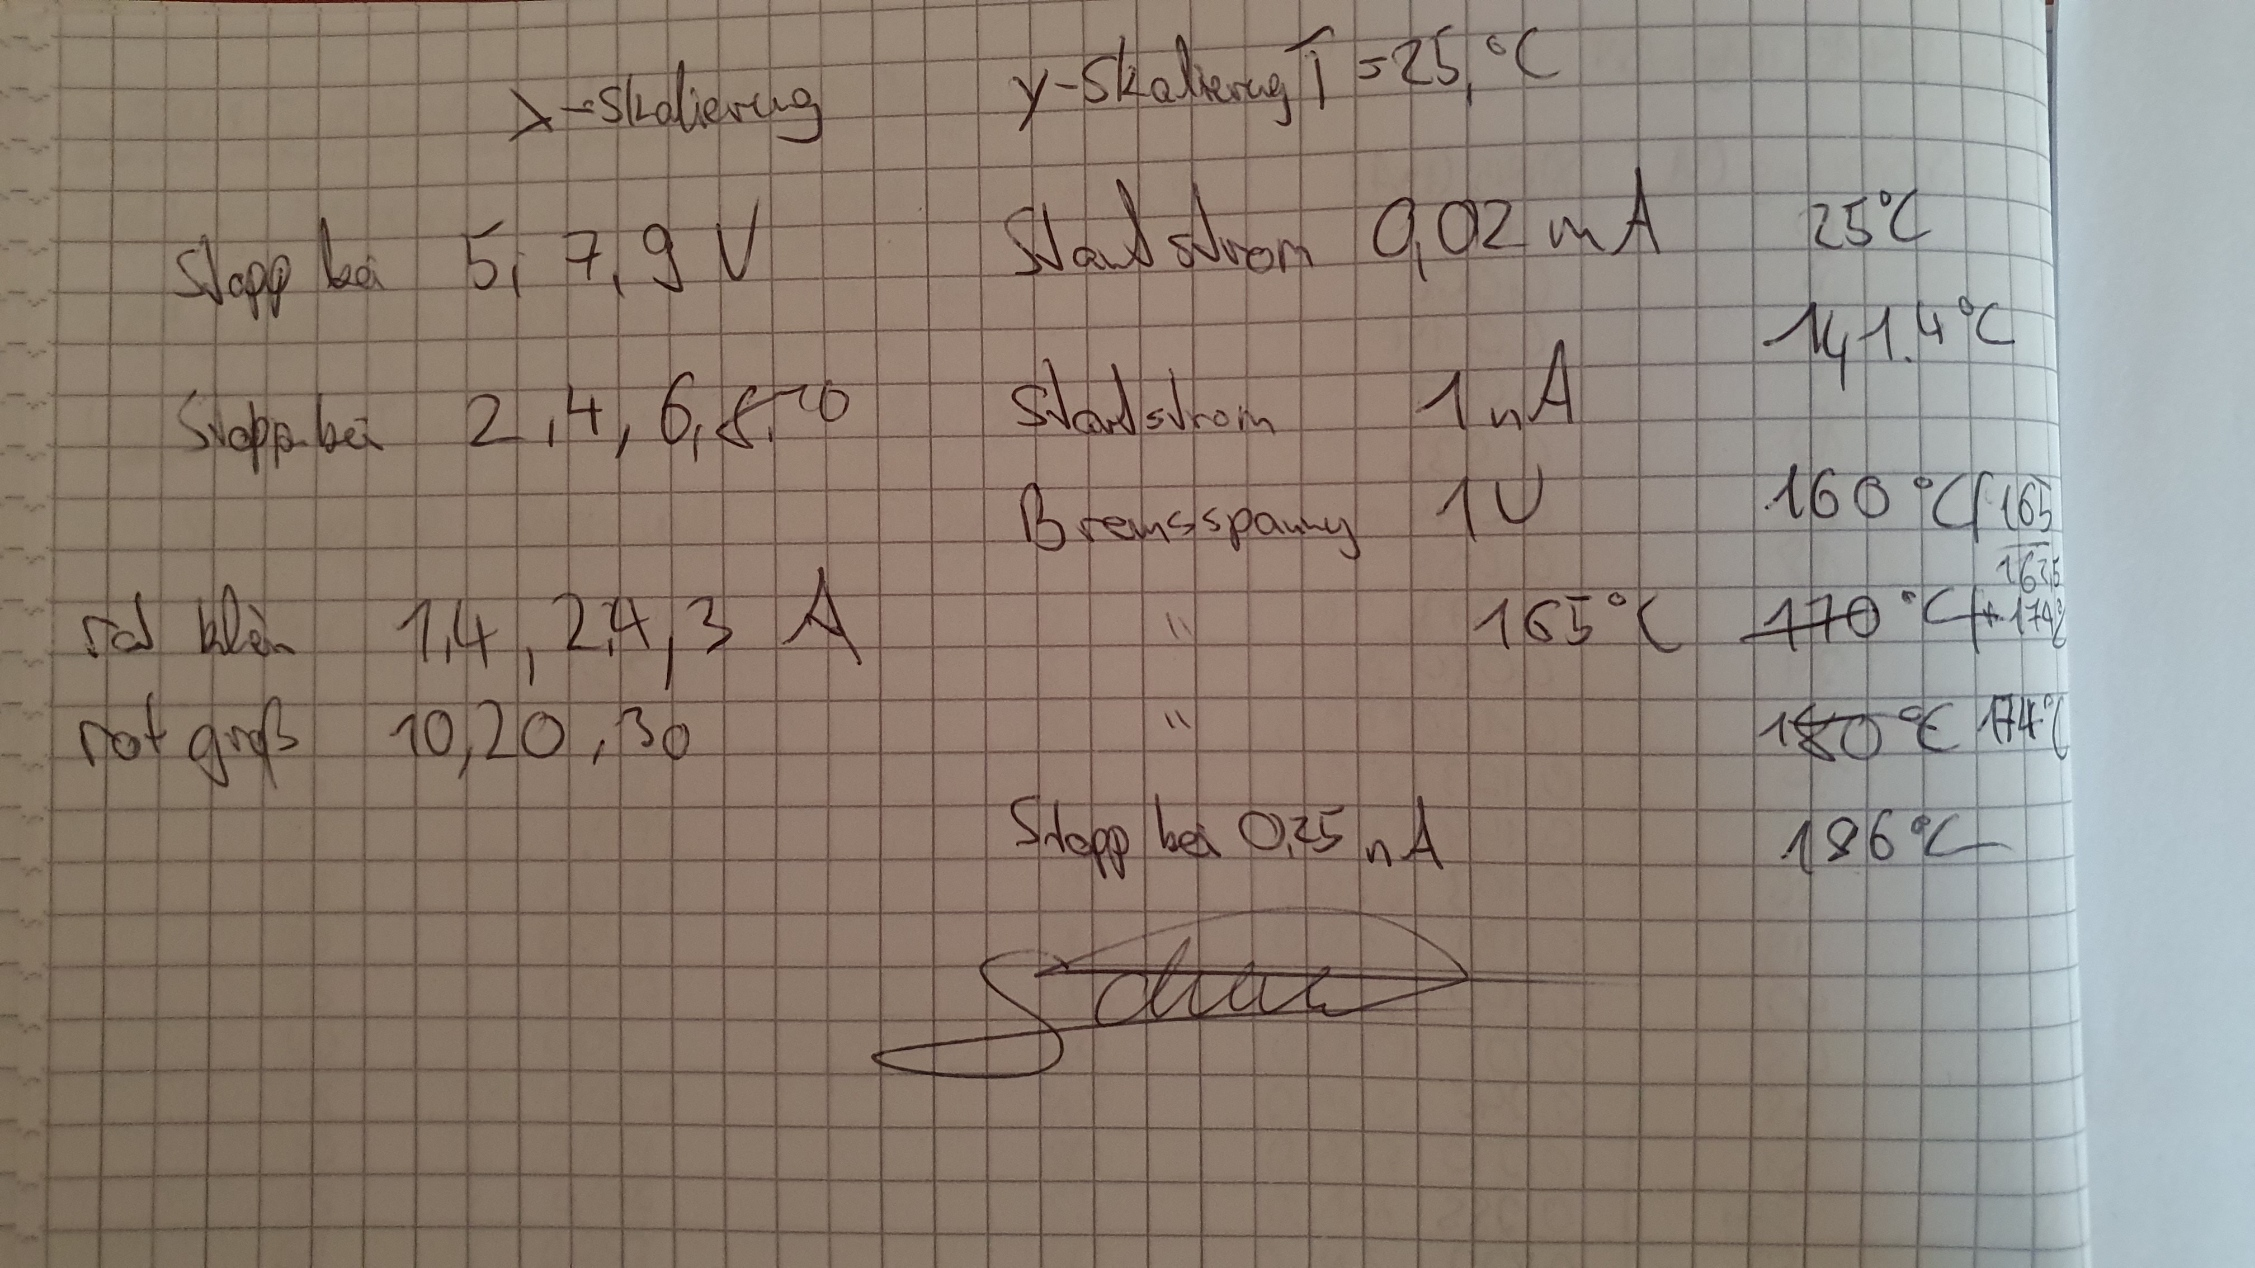
\includegraphics[width=0.9\textwidth]{content/Laborbuch.jpg}
    \centering{Notizen aus dem Laborbuch.}
\end{figure}

%\end{document}
